\documentclass{Configuration_Files/PoliMi3i_thesis}

% CONFIGURATIONS
\usepackage{parskip} % For paragraph layout
\usepackage{setspace} % For using single or double spacing
\usepackage{emptypage} % To insert empty pages
\usepackage{multicol} % To write in multiple columns 
\setlength\columnsep{15pt} % Column separation in executive summary
\setlength\parindent{0pt} % Indentation

\raggedbottom  

% PACKAGES FOR TITLES
\usepackage{titlesec}
\titlespacing{\section}{0pt}{3.3ex}{2ex}
\titlespacing{\subsection}{0pt}{3.3ex}{1.65ex}
\titlespacing{\subsubsection}{0pt}{3.3ex}{1ex}
\usepackage{color}

% PACKAGES FOR LANGUAGE AND FONT
\usepackage[english]{babel} % The document is in English  
\usepackage[utf8]{inputenc} % UTF8 encoding
\usepackage[T1]{fontenc} % Font encoding
\usepackage[11pt]{moresize} % Big fonts

% PACKAGES FOR IMAGES
\usepackage{graphicx}
\usepackage{transparent} % Enables transparent images
\usepackage{eso-pic} % For the background picture on the title page
\usepackage{subfig} % Numbered and caption subfigures using 
\usepackage{tikz} % A package for high-quality hand-made figures.
\usetikzlibrary{}
\graphicspath{{./Images/}} % Directory of the images
\usepackage{caption} % Coloured captions
\usepackage{xcolor} % Coloured captions
\usepackage{amsthm,thmtools,xcolor} % Coloured "Theorem"
\usepackage{float}

% STANDARD MATH PACKAGES
\usepackage{amsmath}
\usepackage{amsthm}
\usepackage{amssymb}
\usepackage{amsfonts}
\usepackage{bm}
\usepackage[overload]{empheq} % For braced-style 
\usepackage{fix-cm} % To override original LaTeX restrictions 

% PACKAGES FOR TABLES
\usepackage{longtable} % Pacchetto per tabelle multi-pagina
\usepackage{tabularx} % Pacchetto per tabelle adattabili
\usepackage{array} % Pacchetto per definire nuovi tipi di colonna
\usepackage{caption} % Pacchetto per gestire la didascalia
\usepackage{geometry}
\usepackage{colortbl}

% PACKAGES FOR ALGORITHMS (PSEUDO-CODE)
\usepackage{algorithm}
\usepackage{algorithmic}

% PACKAGES FOR REFERENCES & BIBLIOGRAPHY
\usepackage[colorlinks=true,linkcolor=black,anchorcolor=black,citecolor=black,filecolor=black,menucolor=black,runcolor=black,urlcolor=black]{hyperref} % Adds clickable links at references
\usepackage{cleveref}
\usepackage[square, numbers, sort&compress]{natbib} % Square brackets, citing references with numbers, citations sorted by appearance in the text and compressed
\bibliographystyle{abbrvnat} % You may use a different style adapted to your field

% OTHER PACKAGES
\usepackage{pdfpages} % To include a pdf file
\usepackage{afterpage}
\usepackage{lipsum} % DUMMY PACKAGE
\usepackage{fancyhdr} % For the headers
\fancyhf{}

\usepackage{listings}
\usepackage{xcolor}
\lstdefinelanguage{Alloy}{
    keywords={sig, module, abstract, extends, fact, fun, pred, all, some, one, disj, let, set, implies, in, and, or, not, no, sum},
    keywordstyle=\color{blue}\bfseries,
    sensitive=true,
    comment=[l]//,
    morecomment=[s]{/*}{*/},
    commentstyle=\color{green}\itshape,
    stringstyle=\color{red}\ttfamily,
    morestring=[b]",
}

\lstset{
    language=Alloy,
    basicstyle=\ttfamily\small,
    %backgroundcolor=\color{lightgray}, % Optional background color
    numbers=left, % Line numbers on the left
    numberstyle=\tiny\color{gray},
    frame=single, % Frame around the code block
    breaklines=true, % Automatically break long lines
}

% Define blue color typical of polimi
\definecolor{bluepoli}{cmyk}{0.4,0.1,0,0.4}

% Custom theorem environments
\declaretheoremstyle[
  headfont=\color{bluepoli}\normalfont\bfseries,
  bodyfont=\color{black}\normalfont\itshape,
]{colored}

% Set-up caption colors
\captionsetup[figure]{labelfont={color=bluepoli}} % Set colour of the captions
\captionsetup[table]{labelfont={color=bluepoli}} % Set colour of the captions
\captionsetup[algorithm]{labelfont={color=bluepoli}} % Set colour of the captions

\theoremstyle{colored}
\newtheorem{theorem}{Theorem}[chapter]
\newtheorem{proposition}{Proposition}[chapter]

% Enhances the features of the standard "table" and "tabular" environments.
\newcommand\T{\rule{0pt}{2.6ex}}
\newcommand\B{\rule[-1.2ex]{0pt}{0pt}}

% Pseudo-code algorithm descriptions.
\newcounter{algsubstate}
\renewcommand{\thealgsubstate}{\alph{algsubstate}}
\newenvironment{algsubstates}
  {\setcounter{algsubstate}{0}%
   \renewcommand{\STATE}{%
     \stepcounter{algsubstate}%
     \Statex {\small\thealgsubstate:}\space}}
  {}

% New font size
\newcommand\numfontsize{\@setfontsize\Huge{200}{60}}

% Title format: chapter
\titleformat{\chapter}[hang]{
\fontsize{50}{20}\selectfont\bfseries\filright}{\textcolor{bluepoli} \thechapter\hsp\hspace{2mm}\textcolor{bluepoli}{|   }\hsp}{0pt}{\huge\bfseries \textcolor{bluepoli}
}

% Title format: section
\titleformat{\section}
{\color{bluepoli}\normalfont\Large\bfseries}
{\color{bluepoli}\thesection.}{1em}{}

% Title format: subsection
\titleformat{\subsection}
{\color{bluepoli}\normalfont\large\bfseries}
{\color{bluepoli}\thesubsection.}{1em}{}

% Title format: subsubsection
\titleformat{\subsubsection}
{\color{bluepoli}\normalfont\large\bfseries}
{\color{bluepoli}\thesubsubsection.}{1em}{}

% Shortening for setting no horizontal-spacing
\newcommand{\hsp}{\hspace{0pt}}

\makeatletter
% Renewcommand: cleardoublepage including the background pic
\renewcommand*\cleardoublepage{%
  \clearpage\if@twoside\ifodd\c@page\else
  \null
  \AddToShipoutPicture*{\BackgroundPic}
  \thispagestyle{empty}%
  \newpage
  \if@twocolumn\hbox{}\newpage\fi\fi\fi}
\makeatother

%For correctly numbering algorithms
\numberwithin{algorithm}{chapter}

%------------------------
%	BEGIN OF YOUR DOCUMENT
%-------------------------

\begin{document}

\fancypagestyle{plain}{%
\fancyhf{} % Clear all header and footer fields
\fancyhead[RO,RE]{\thepage} %RO=right odd, RE=right even
\renewcommand{\headrulewidth}{0pt}
\renewcommand{\footrulewidth}{0pt}}

%-------------------
%	TITLE PAGE
%-------------------
\pagestyle{empty} %
\frontmatter 
\puttitle{
	title=Students \& Companies, 
	name= Paone A. Pasqual M. Restelli M., 
	course=Software Engineering 2 Project,
	advisor= Prof. Camilli Matteo,
	academicyear={2024-25},  
} 
\startpreamble
\setcounter{page}{1} 

% TABLE OF CONTENTS
\thispagestyle{empty}
\tableofcontents % Table of contents 
\thispagestyle{empty}
\cleardoublepage

%--------------------
%	THESIS MAIN TEXT
%--------------------
\addtocontents{toc}{\vspace{2em}} 
\mainmatter 



% -----------------------
% INTRODUCTION SECTION
% -----------------------
\chapter{Introduction}

\section{Purpose}
As the demand for skilled interns in various industries continues to rise, providing students with relevant internship opportunities is essential for their professional growth. 
Traditionally, students often struggle to find internships that match their skills, experiences, and career aspirations, while companies face challenges in sourcing qualified candidates. 
Students\&Companies (S\&C) aims to bridge this gap by creating a dynamic platform that helps the matching of university students with companies offering internships tailored to their profiles.

S\&C provides a unified framework for students to search for internships, allowing them to showcase their CVs and preferences. 
Companies can advertise their internship opportunities, detailing the required skills, tasks, and benefits offered.
The platform employs sophisticated recommendation mechanisms, utilizing keyword searches and statistical analyses to enhance the matching process, thereby ensuring a better fit between students and internships.
Furthermore, S\&C allows for the tracking of the interview process and provides constructive suggestions for improving project descriptions and CVs. Additionally, it facilitates the management of complaints from universities, enhancing overall communication and collaboration. 

The main goals of the platform are the following:

\subsection{Goals}

[G1] Companies should be able to advertise the internships they want to offer 

[G2] Students should be able to look for internships 

[G3] Students should be able to be informed about internships that can be interesting  

[G4] Companies should be able to be informed about the availability of a student's CVs 

[G5] Students and Companies should be able to accept a recommendation of a possible match

[G6] Students and Companies should be able to establish contact and participate in an interview

[G7] Students and Companies should be able to provide feedback and suggestions on the provided recommendations

[G8] Students and companies should be able to receive suggestions regarding how to make their submissions (project descriptions for companies and CVs for students)

[G9] Students and companies should be able to keep track of the matchmaking and internship processes

[G10] Students and Companies should be able to complain, communicate problems, and provide information on the status of internships

[G11] Universities should be able to monitor internships

[G12] Universities should be able to handle complaints


\section{Scope}
Students\&Companies (S\&C) is a platform whose aim is to connect students who are looking for internships with compa 

\subsection{World Phenomena}
[WP1] Students prepare their CVs

[WP2] Students want to take part in an internship experience 

[WP3] Companies want to employ a student as an intern 

[WP4] Companies interview possible candidates 

[WP5] Students inform their university about the internship when it's in the course

[WP6] Companies choose the best candidate

\subsection{Shared Phenomena}

\subsubsection{World-controllled}
[SP1] Students upload their CVs

[SP2] Students go through available internships

[SP3] Companies advertise their internship

[SP3] Students accept the recommendation of an internship

[SP4] Companies accept the recommendation of a student

[SP6] Companies use the system to manage interviews

[SP7] Companies use the system to finalize the selections

[SP8] Universities monitor the situation of the internship

[SP9] Universities handle complaints

[SP10] Students and companies use the system to complain, communicate problems, and provide information about the internship status.

\subsubsection{Machine-controllled}
[SP11] The system informs students when an interesting internship becomes available

[SP12] The system informs companies when an interesting CV becomes available

[SP13] The system asks students and companies to provide feedback and suggestion

[SP14] The system provides suggestions both to companies and students on how to make submissions

[SP15] The system provides a mechanism to monitor the process and internship


\section{Definitions, Acronymous, Abbreviations}
\begin{table}[H]
\centering
\begin{tabular}{|l|l|}
\hline
\textbf{Abbreviation} & \textbf{Description} \\ \hline
RASD & Requirements Analysis \& Specification Document \\ \hline
G* & Goal \\ \hline
WP* & World phenomena \\ \hline
SP* & Shared phenomena \\ \hline
D* & Domain assumption \\ \hline
R* & Functional requirement \\ \hline
UC* & Use case \\ \hline
S\&C & Students \& Companies \\ \hline
ST & Students \\ \hline
COM & Companies \\ \hline
UML & Unified Modelling Language \\ \hline
UI & User Interface \\ \hline
\end{tabular}
\caption{List of Definitions, Acronymous, and Abbreviations}
\label{table:abbreviations}
\end{table}

  
\section{Revision History}

\begin{itemize}
    \item Version 1.0 (04/11/2024)
\end{itemize}

\section{Reference Documents}

The document is based on the following materials:

\begin{itemize}
    \item IEEE Standard Documentation For RASD
    \item The specification of the RASD and DD assignment of the Software Engineering II course a.a. 2024/25 
    \item Slides of the course on WeBeep
\end{itemize}


\section{Document Structure}

\begin{enumerate}
    \item  \textbf{Introduction}: it aims to give a brief description of the project. In particular, it’s focused on the reasons and the goals that are going to be achieved with its development;
 
    \item \textbf{Overall Description}: it is a high-level description of how the system works with a detailed explanation of the phenomena that involve the world, the machine, or both, there is also the domain description with its assumptions;
 
    \item \textbf{Specific Requirements}: in this section, there is a detailed analysis of the requirements needed to achieve the goals. Moreover, it contains more information useful for developers (i.e constraints about HW and SW);
    
    \item \textbf{Formal analysis}: it’s a formal description of the world phenomena using Alloy;

    \item  \textbf{Effort spent}: it shows the time spent to realize this document organized by section;

    \item  \textbf{References}: it contains the references to any documents and software used to write this paper.
    
\end{enumerate}
\chapter{Overall Description}
This section is devoted to an overall description of every part of the system.

\section{Product Perspective}
\subsection{Scenarios}

\begin{enumerate}
    \item \textbf{A student creates an account}

    Mario Rossi, a university student eager to participate in an internship, is unsure of how to directly contact companies. 
    
    After learning about Students\&Companies, he decides to explore the platform and create an account. Searching for the site in his browser, Mario arrives at a login page, where he sees an option to create a new account if he is not yet registered. He clicks on this option and follows the account creation steps: entering his email, first name, last name, and date of birth.
    
    Upon completing these basic details, Mario is presented with additional options to enhance his profile, such as uploading a CV and adding a brief personal description. However, he decides to skip this step for now, intending to add these details later, as he is currently focused on just exploring what the platform looks like.
    \item \textbf{A student uploads their CV}

    After exploring the site and deciding he would like to be contacted by companies, Mario decides it’s time to enhance his profile by uploading his CV. To do this, he follows a series of steps:

    First, Mario clicks on his profile to access his personal information. Within his profile, he finds a button labeled "Add your CV" and selects it. This action opens his computer's file browser, where he locates his CV and clicks "Upload." 
    
    Once the file is uploaded, Mario clicks "Publish," making his CV visible to anyone who views his profile.

    This update is also noted by the platform, which analyzes the information within his CV. Based on this analysis, the platform notifies relevant companies who may be searching for profiles similar to Mario's, informing them of the availability of a new candidate.
    \item \textbf{A company advertizes their internship}
    
    TechSolutions, a company seeking interns for a new project, is already familiar with Students\&Companies and has an active account on the platform.
    
    To advertise their open internship position, they navigate to their company profile and select the "Add a new project description" button. This opens a page where they can enter a detailed description of the job responsibilities and the type of student profile they are seeking. 
    
    Once they have completed the description, they click "Publish," making the internship opportunity visible to all visitors to their profile.

    The platform then analyzes this new project listing and notifies students whose profiles match the requirements for the position. 
    
    
    Additionally, students visiting the profile will now be able to click an "Apply" button next to the project description to submit their applications directly, even if they have not received a notification from the system.
    \item \textbf{A student accepts a recomendation}

    Mario, a student with a profile and CV on Students\&Companies, receives a recommendation email from the platform, notifying him of an internship opportunity at a company that aligns with his interests.
   
    In this email, Mario has the option to click on a "See Recommendation" button, which redirects him to his profile. There, he finds a new message containing a link to the company’s account.

    Mario reviews the company’s profile and examines the project that the platform has recommended to him. If he finds it appealing, he can return to the message on his profile and click the "Accept Recommendation" button.

    This action is then flagged by the system to the company, allowing them to contact Mario directly through the platform to coordinate the next steps in the selection process.
    \item \textbf{A company uses the system to manage the interview}

    TechSolutions, having established contact with student Mario Rossi via Students\&Companies, begins the preselection process facilitated by the platform.

    The first step offered by Students\&Companies is for the company to set up a structured questionnaire through Microsoft Forms, featuring predefined questions that Mario must answer. This allows the company to gain a clearer understanding of Mario’s interests, skills, and suitability for the role. If TechSolutions finds his responses satisfactory, they will proceed to the next stage of the interview process; otherwise, they will inform Mario that he has been excluded from further consideration.

    Should they decide to proceed, TechSolutions can initiate a direct chat with Mario to arrange an interview. The interview can be held in person if Mario is able to travel to the location, or via video call if he is unable to attend in person.

    During the interview itself, the company may choose to use additional tools provided by Students\&Companies, such as a shared digital whiteboard for collaborative problem-solving, the ability to share relevant files or documents in real-time, or access to preloaded questions or skills assessments within the system. These tools can facilitate a more interactive and efficient interview experience.

    \item \textbf{A company uses the system to finalize the selection}

    \item \textbf{Students are asked to provide feedback and suggestions}

    \item \textbf{Companies recieve a suggestion on how to make their project description more appealing}

    \item \textbf{A student makes a complaint}

    \item \textbf{A university monitors the situation of an internship}

    \item \textbf{A university handles a complaint}
\end{enumerate}


\subsection{Class diagram}
a

\subsection{State diagrams}
a

\section{Product Functions}
a


\section{User charatteristic}

Università??

There are two types of registered users in S\&C: Students (STs) and Companies (COMs). Each user type has distinct characteristics and roles within the platform:

\begin{itemize}
    \item \textbf{STs}: Students use S\&C to find a company offering internships. To access the platform, they must have a device with an internet connection and an account that includes their email and personal data. Once registered, students can browse available internships, apply for them, and participate in interviews with 
    companies

    \item \textbf{COMs}:  Companies join S\&C to find students suitable for internships. To use the platform, they need a device with an internet connection and an account that includes their email and company information. Through S\&C, companies can view student applications, schedule interviews, and select candidates for internships.
\end{itemize}

Both STs and COMs must register with the platform to access its services, enabling seamless communication between students seeking internships and companies offering opportunities.

\section{Assumptions, dependencies, constraints}
\textbf{[DA1] }Students and companies need to have a device and an internet connection (?)

\textbf{[DA2]} Companies need to have detailed internship descriptions

\textbf{[DA3]} Students need to have a CV

\textbf{[DA4]} Students need to be enrolled at a university 

\textbf{[DA5]} Students need to create an account on S\&C as students.

\textbf{[DA6]} Companies need to create an account on S\&C as Companies.

\textbf{[DA7]} Universities need to create an account on S\&C as Universities.

\textbf{[DA8]} Companies need to be able to conduct an interview

\textbf{[DA9]} Companies need to be able to evaluate an interview

\textbf{[DA10]} Universities need to be informed about a current student's internship

\textbf{[DA11]} Universities need to be able to communicate with Students and Companies


\chapter{Specific Requirements}
This section provides a detailed description of the various types of requirements the system must address to achieve all the functionalities outlined. These requirements are essential to ensure the platform operates efficiently, and securely meeting users needs. 

\section{External Interface Requirements}
\subsection{User Interfaces}
The Students\&Companies (S\&C) user interface will be a web app developed to be used by both STs and COMs. It will be accessible to anyone with a device equipped with an internet browser and a reliable internet connection. The platform will provide an intuitive and user-friendly experience, ensuring that users can easily navigate and access its features regardless of their device or operating system.

\subsection{Hardware Interfaces}
The system will be accessible from every device with an Internet Browser to access the website and a reliable Internet connection. The User is free to choose his device like a computer, a tablet, or a smartphone.

The system will be accessible from any device with an internet browser and a reliable internet connection. Users can choose their preferred device, whether it is a computer, tablet, or smartphone. This ensures flexibility and convenience, allowing users to access the platform from anywhere and at any time.

\subsection{Software Interfaces}
The system requires an API to facilitate email sending. These emails can include, for instance, 2FA (two-factor authentication) confirmations or general notifications. This functionality is essential to ensure secure user authentication and to keep users informed about important updates and communications through email.
 
\subsection{Communication Interfaces}
The communication interfaces needed by the system are the HTTPS (Hypertext Transfer Protocol Secure) protocol and the Mail System Transfer Protocol (SMTP). 

\begin{itemize}
    \item \textbf{HTTPS} will be used to ensure secure communication between the client and the server, protecting data integrity and confidentiality during transactions such as login, registration, and other sensitive operations.
    
    \item \textbf{SMTP} will be used for sending emails, enabling the system to handle tasks such as sending account 2FA confirmations, notifications, and other user-related communications efficiently and securely.

\end{itemize}

\section{Functional Requirements}

\textbf{[R1]} The system allows unregistered users to create an account

\textbf{[R2]} The system allows students to upload their CV

\textbf{[R3]} The system allows companies to publish new internships

\textbf{[R4]} The system allows companies to add a description to their internships

\textbf{[R5]} When students want to do a proactive research, the system allows them to go through the available internships

\textbf{[R6]} When doing a search the system allows users to filter internships by a key (?)

\textbf{[R7]} When finding an internship that suits their interests, the system allows students to apply for it. 

\textbf{[R8]} When a new internship that might interest some students becomes avaible, the system notifies them.

\textbf{[R9]} When a student's CV that corresponds to a company's needs becomes available the system informs them. 

\textbf{[R10]} The system allows students to accept a recommendation, applying for that particular internship. 

\textbf{[R11]} The system allows companies to accept a recommendation, inviting the candidate that was proposed.

\textbf{[R12]} The system allows students to accept an invitation of a company for a particular internship, applying for it.

\textbf{[R13]}  When the two parties have accepted a recommendation, or when the company has accepted an application received, the system allows them to establish a contact

\textbf{[R14]} When conducting an interview, the system supports the companies with the interview process

\textbf{[R15]} When conducting an interview, the system supports the companis with the finalization of the selection

\textbf{[R16]} The system allows students and companies to provide feedback and suggestions to feed statistical analysis.

\textbf{[R17] }The system provides suggestions to students regarding how to make their CVs more appealing

\textbf{[R18]} The system provides suggestions to companies regarding how to make their project descriptions more appealing

\textbf{[R19]} During the matchmaking process, the system allows all users to keep track of its execution and outcome

\textbf{[R20]} During the internship the system allows all interested parties to monitor it

\textbf{[R21]} During and ongoing internship, the system allows all users to complain 

\textbf{[R22]} During and ongoing internship, the system allows all users to communicate problems 

\textbf{[R23]} During and ongoing internship, the system allows all users to provide information on its status

\textbf{[R24]} When reports or complaints about the status of an ongoing internship are made, the system allows Universities to see them.

\textbf{[R25]} When complaints about the status of an ongoing internship are made, the system allows Universities to handle them.

\pagebreak

\subsection{Use case diagrams}

\begin{figure}[H]
    \centering
    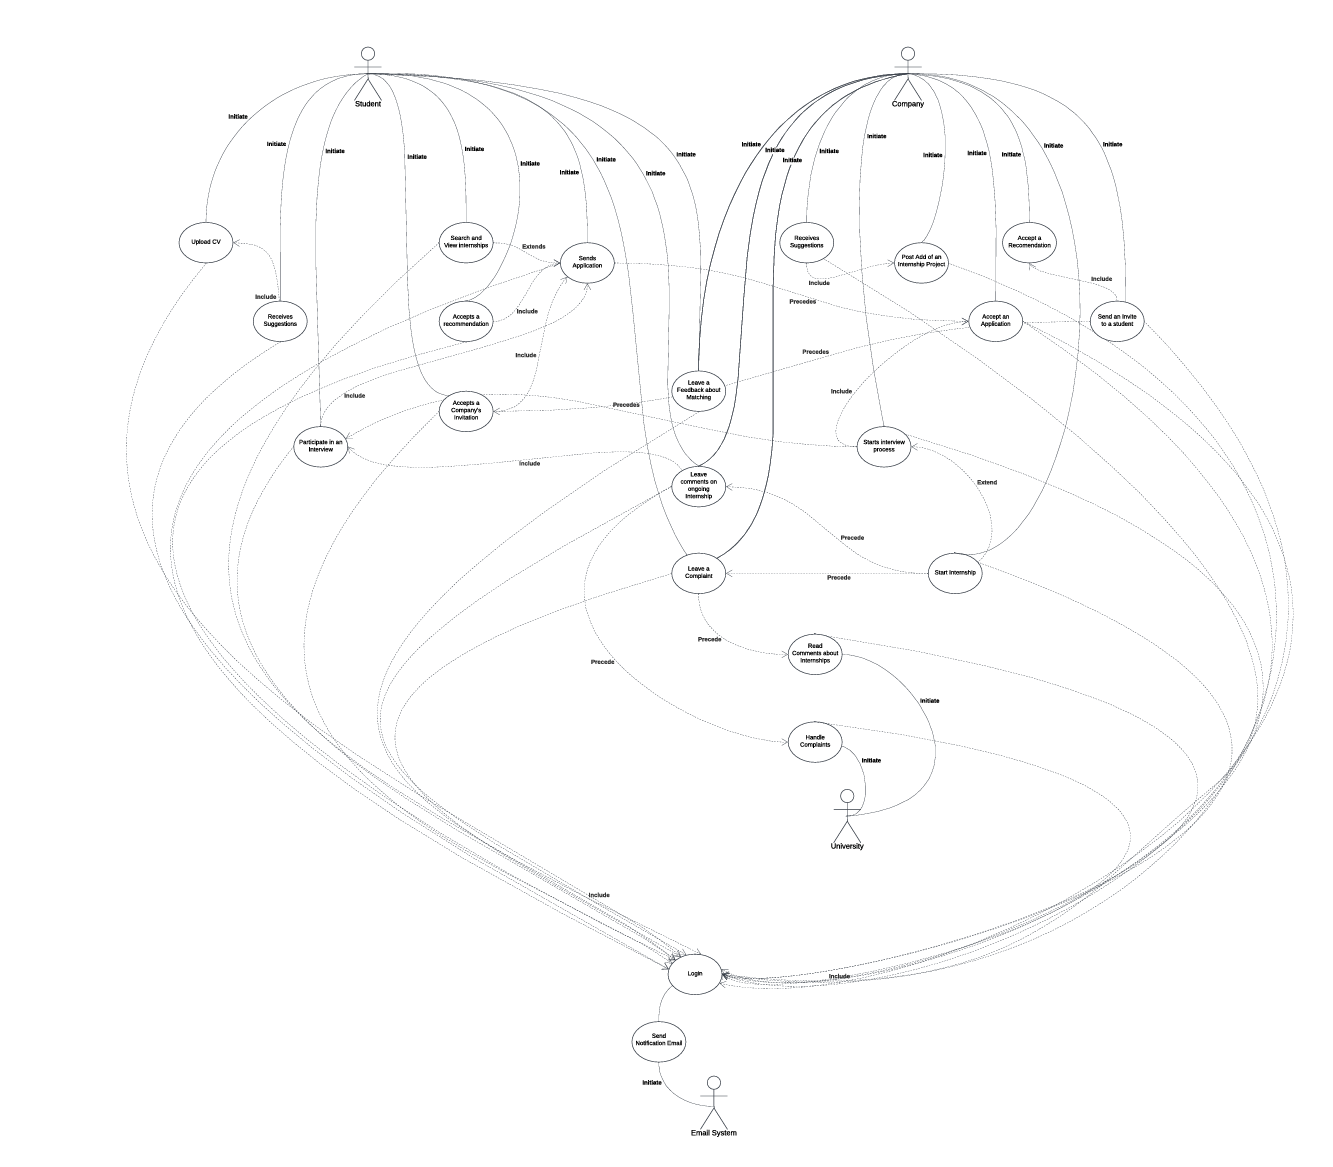
\includegraphics[width=1\linewidth]{RASD//Images/usecase.png}
    \caption{Use case diagrams}
    \label{fig:enter-label}
\end{figure}


\subsection{Use cases}
tabella per ogni uc e poi aggiungi i sequence diagrams
\begin{itemize}
\item Students create an account
\item Companies create an account
\item Student searches and applies for an internship
\item Student recieves an internship recomendation (accept / decline)
\item Company recieves a student’s recomendation (invite students + accept)
\item Interview Process
\item Student receives suggestions on CV
\item Company receives suggestions on Add
\item User leaves feedback
\item User leaves comments on ongoing internship
\item University monitors and handles complaints
\end{itemize}

Come gestiamo i reply messages? mettiamo il ritorno ogni volta che il sistema cambia pagina? (ci vuole la freccia tratteggiata di ritorno ogni volta che facciamo un operazione per segnalare l'azione del sistema in risposta a quell'operazione.)

\textbf{UC1}

\begin{longtable}{|p{0.3\textwidth}|p{0.65\textwidth}|}
\hline
\textbf{Name} & Student creates an account \\
\hline
\textbf{Actor} & Student\\
\hline
\textbf{Entry Condition} & The Student has a valid institutional email, the student enters the platform for the first time.\\
\hline
\textbf{Event Flow} & 
\begin{enumerate}
    \item The student opens the platform homepage.
    \item The student selects the "Sign up" in the "Student's Account" option.
    \item The platform displays a registration form.
    \item The student inputs the following details:	institutional email address. legal name, birth date, location of residence.
    \item The student clicks the "Sign-Up" button
    \item The system verifies the email address format, and checks for duplicate email addresses in existing accounts.
    \item  If validations pass the system generates a username based on the student’s legal name.
    \item The platform sends a verification email to the provided email address.
    \item The student opens the verification email and clicks the provided link to validate their identity.
    \item Upon successful verification, the system creates and activates the account.
    \item The system sends a welcome message, inviting the student to upload their CV if desired.
    \item  If the student decides to upload a CV they click on the message, which redirects them to the CV upload page.
    \item The student uploads their CV and confirms the upload.
    \item If the student chooses not to upload a CV, they dismiss the message by clicking the "X" button.
\end{enumerate} \\
\hline
\textbf{Exit Condition} & 
1. The student’s account is created, verified, and activated.

2. Optional: The student’s CV is uploaded.\\
\hline
\textbf{Exception} & 
1. If the email address is already associated with an existing account, the system displays an error message, the student is redirected to the login page to access their existing account.	

2. If the email address is invalid, the system displays an error message and requires the student to re-enter the email address.	

3. If the student fails to confirm their identity within a set time (e.g., 24 hours), the account creation process is canceled.\\
\hline
\end{longtable}

\textbf{UC2}

\begin{longtable}{|p{0.3\textwidth}|p{0.65\textwidth}|}
\hline
\textbf{Name} & Company creates an account \\
\hline
\textbf{Actor} & Company\\
\hline
\textbf{Entry Condition} & The Company has a valid email addess, the company enters the platform for the first time. \\
\hline
\textbf{Event Flow} & 
\begin{enumerate}
    \item The company opens the platform homepage.
    \item The company selects the "Sign up" in the "Company's Account" option.
    \item The platform displays a registration form.
    \item The company inputs the following attributes: email address, company name, location.
    \item The company clicks the "Sign-Up" button.
    \item The system verifies the email address format and checks for duplicate email addresses in existing accounts.
    \item If validations pass, the system generates a username based on the company name.	
    \item The platform sends a verification email to the provided email address.
    \item The company opens the verification email and clicks the provided link to validate their identity.
    \item Upon successful verification, the system creates and activates the account.
    \item The system sends a welcome message inviting the company to upload project descriptions.
    \item  The company clicks the message.
    \item The system redirects them to a page to upload project descriptions.
    \item  The company writes and publishes project descriptions using the provided form.
\end{enumerate} \\
\hline
\textbf{Exit Condition} & 
1. A new account is created, verified, and activated.

2. The company has uploaded their first project descriptions.\\
\hline
\textbf{Exception} & 
1. If the email address is already associated with an existing account, the system displays an error message and the company is redirected to the login page to access their existing account.	

2. If the email address is invalid, the system displays an error message and requires the company to re-enter the email address.	

3. If the company fails to confirm their identity within a set time (e.g., 24 hours), the account creation process is canceled.\\
\hline
\end{longtable}

\textbf{UC3}

\begin{longtable}{|p{0.3\textwidth}|p{0.65\textwidth}|}
\hline
\textbf{Name} &  Student searchs and applies for an internship\\
\hline
\textbf{Actor} &  Student, Company\\
\hline
\textbf{Entry Condition} &  The student is correctly logged in and has decided he wants to look for an internship. He is on the home page of S\&C.\\
\hline
\textbf{Event Flow} &  
\begin{enumerate}
    \item  The student clicks on the "Global" button on the homepage.
    \item S\&C displays the "Global" page with a list of internships available.
    \item The student scrolls through and reads the list of available internships.
    \item If the student identifies an internship of interest they click on the internship's title.
    \item S\&C displays the project description page for that internship.
    \item The student reads the description.
    \item If the student is still interested in applying they click on the "Apply" button.
    \item S\&C sends the application, along with the student's profile, to the company managing the internship.
    \item The system displays a confirmation message to the student, confirming the application has been sent.
    \item If the student is not interested after reading the description, they click the "Back" button to return to the list of available internships.
    \item S\&C redirects the student to the correct page.
    \item  If the student does not find any interesting internships in the list they close the browser, ending the session.
\end{enumerate} \\
\hline
\textbf{Exit Codition} &  
1. The student successfully submits an application and receives confirmation.

2. The student exits without applying for an internship.\\
\hline
\textbf{Exception} &  
1. The "Global" page fails to load due to a technical error.	

2. The internship project description fails to display after the student clicks on a title.

3. The application submission fails due to an error, and the system provides an appropriate error message.	

4. The student encounters internet connectivity issues, preventing them from completing the process.\\
\hline
\end{longtable}


\textbf{UC4}

\begin{longtable}{|p{0.3\textwidth}|p{0.65\textwidth}|}
\hline
\textbf{Name} &  Student recieves an internship recomendation\\
\hline
\textbf{Actor} &  Student, Company\\
\hline
\textbf{Entry Condition} &  The student has a valid email account and is able to log into the system. The student has uploaded a CV on his profile.\\
\hline
\textbf{Event Flow} &  
\begin{enumerate}
\item S\&C finds a match between a student and a company based on the student's CV and the company’s project description..
\item S\&C sends an email to the student notifying them of the internship recommendation..
\item The student recieves an email and clicks on the "Go to Recommendation" button.
\item S\&C redirects the student to their profile page, displaying the recommendation details, including the project description.
\item The student reviews the project description, if the student accepts the recommendation they click the "Apply" button.
\item S\&C notifies the company that the recommended student has applied for the position.
\item The system confirms the application to the student.
\item If the student rejects the recommendation, they click the "Reject Recommendation" button.
\item S\&C removes the match from its database.
\item S\&C notifies the company they matched with that the recomendation has been rejected by the student. 
\end{enumerate}
\\
\hline
\textbf{Exit Codition} & 
1. The student has successfully applied to the internship and received confirmation.

2. The student has exited the process without applying.\\
\hline
\textbf{Exception} &  
    1. The student does not see the email in time, and the internship application window has already closed when they attempt to apply.	
    
    2. The email fails to reach the student due to a technical issue.	
    
    3. The link in the email to the recommendation page is broken or inaccessible.\\
\hline
\end{longtable}



\textbf{UC5}

\begin{longtable}{|p{0.3\textwidth}|p{0.65\textwidth}|}
\hline
\textbf{Name} &  Company recieves a student's recomendation\\
\hline
\textbf{Actor} &  Company, Student\\
\hline
\textbf{Entry Condition} &  
1. The company has a valid email account and is able to log into the system.

2. The company has uploaded at least one project description on their profile.\\
\hline
\textbf{Event Flow} &  
\begin{enumerate}
\item S\&C identifies a match between a student and a company based on the uploaded project description and student CV.	
\item S\&C sends an email to the company notifying them of the recommendation.
\item  The company’s employee receives the email and clicks on the "Go to Recommendation" button.
\item  The system redirects them to their profile page, displaying the recommendation details, including a link to the student's profile.
\item The company’s employee reviews the student’s CV, If the employee is interested in the student:
\item  If the student has already applied, the company clicks the "Accept" button.
\item S\&C notifies the student that their application has been accepted, and contact between the two parties is established.
\item  If the student has not applied, the company clicks the "Invite" button.
\item S\&C sends a notification to the student requesting that they submit an application.
\item If the employee is not interested in the student:
\item If the student has already applied, the company clicks the "Reject Application" button.
\item S\&C notifies the student that their application has been rejected.
\item  If the student has not applied, the company clicks the "Reject Recommendation" button. (Lo mettiamo o semplicemente ignora?)
\item S\&C removes the match from the system.
\item S\&C notifies the student they matched with that the recomendation has been rejected by the company. 
\end{enumerate}\\
\hline
\textbf{Exit Codition} &  
1. Contact is successfully established between the student and the company.

2. The student is notified of a rejected match.\\
\hline
\textbf{Exception} &  
1. The email fails to reach the company due to a technical issue.

2. The link in the email to the recommendation page is broken or inaccessible.	

3. The company’s employee does not respond to the email or does not review the recommendation on the platform.	\\
\\
\hline
\end{longtable}



\textbf{UC6}

\begin{longtable}{|p{0.3\textwidth}|p{0.65\textwidth}|}
\hline
\textbf{Name} &  Interview\\
\hline
\textbf{Actor} &  Student, Company\\
\hline
\textbf{Entry Condition} &  
\begin{itemize}
    \item A student has been matched with a company.
    \item The company and student have been notified of the match.
    \item The company has initiated contact by either accepting the student's application or requesting an interview.
\end{itemize} 
\\
\hline
\textbf{Event Flow} &  
\begin{enumerate}
    \item The company contacts the student through the platform..
    \item The student receives a notification from the platform that a company is requesting to initiate contact.
    \item The student accepts, and they begin the interview process.
    \item The company may use platform tools, such as questionnaires, to pre-assess the student's qualifications before scheduling the interview.
    \item The student completes the pre-assessment through the system, providing relevant information and responses.
    \item Upon reviewing the pre-assessment, the company decides whether to move forward with the interview process. If they decide to proceed, the company proposes an interview date and time for the student to consider.
    \item The student reviews the proposed interview details and, if they are available, accepts the scheduled date and time.
    \item If the student is unavailable at the proposed time, they request the company to reschedule the interview.
    \item This process repeats until both parties agree on a time for the interview.
    \item Once a suitable time has been found, the system confirms the interview date and time with both the student and the company.
    \item The student and company receive a reminder notification prior to the interview.
    \item The company and student conduct the interview (this could be through the platform or an external tool as specified).
    \item After the interview, the company uses some tools offered by the system to help with the selection process.
    \item Once they have made a choice, they send a notification to the student with thier choice.
    \item The student is notified whether they have been selected for the internship or not.
    \item If the student is selected, they receive a final confirmation message about joining the internship.
    \item If the student is not selected, they are notified of the rejection and may seek other opportunities.
\end{enumerate} \\
\hline
\textbf{Exit Codition} &  
\begin{enumerate}
    \item The student has either been selected or rejected for the internship.
    \item The company has completed the interview process and provided feedback.
\end{enumerate}\\
\hline
\textbf{Exception} &  
\begin{enumerate}
    \item If the interview cannot be scheduled due to technical issues (e.g., platform or communication failures), the system alerts both parties to reschedule.
    \item If the student fails to respond to the interview request within a set period (e.g., 48 hours), the system sends a reminder, and after another 24 hours, the interview is canceled.
    \item If the company fails to provide feedback or confirmation post-interview, the system will remind the company to complete the process.
\end{enumerate} \\
\hline
\end{longtable}



\textbf{UC7}

\begin{longtable}{|p{0.3\textwidth}|p{0.65\textwidth}|}
\hline
\textbf{Name} &  User leaves feedback\\
\hline
\textbf{Actor} &  User (either student or company representative)\\
\hline
\textbf{Entry Condition} &  
1. The user has a valid email account.

2. The user has an account on S\&C.

3. The user has participated in an internship through S\&C.\\
\hline
\textbf{Event Flow} &  
\begin{enumerate}
    \item The system sends an email to the user requesting feedback about their internship experience.
    \item The user reads the email and decides whether to provide feedback.
    \item If the user chooses to provide feedback, they click the "Leave Feedback" button in the email.
    \item The system redirects them to the S\&C platform, displaying the "Internships to Monitor" page on their profile and an empty space to fill out with the feedback.	
    \item The user writes the feedback.
    \item  If the user does not wish to provide feedback, they ignore the email.
\end{enumerate}\\
\hline
\textbf{Exit Codition} & 
1. The system successfully collects and stores the feedback for analysis.

2. No feedback is received if the user ignores the email.\\
\hline
\textbf{Exception} &  
1. The email fails to reach the user due to a technical issue.	

2. The link to the feedback form in the email is broken or inaccessible.\\
\hline
\end{longtable}

\textbf{UC8}

\begin{longtable}{|p{0.3\textwidth}|p{0.65\textwidth}|}
\hline
\textbf{Name} &  Student recieves suggestion on CV\\
\hline
\textbf{Actor} &  Student\\
\hline
\textbf{Entry Condition} &  
1. The student has an valid email account.

2. The student has an account on S\&C. 

3. The student has uploaded a CV\\
\hline
\textbf{Event Flow} &  
\begin{enumerate}
    \item The student receives an email notification from the system about a new suggestion for their CV.
    \item The student clicks the "See Suggestion" button in the email.
    \item  The system redirects the student to the platform, displaying the page in their profile with the new suggestions.
    \item The student reads the suggestion.
    \item If the student finds the suggestion useful: they navigate to their profile and click the "Change File" button underneath their CV.
    \item The platform opens a page where they can upload a new CV.
    \item The student revises their CV according to the suggestion and reuploads the updated CV to the platform.
    \item If the student does not find the suggestion useful, they ignore the email.
\end{enumerate}\\
\hline
\textbf{Exit Codition} &  
1. The system has a new CV to analyze.

2. The system retains the original CV if no updates are made.\\
\hline
\textbf{Exception} &  
1. The email fails to send.

2. The link to the platform is broken.\\
\hline
\end{longtable}

\textbf{UC9}
\begin{longtable}{|p{0.3\textwidth}|p{0.65\textwidth}|}
\hline
\textbf{Name} &  Company recieves suggestion on project description\\
\hline
\textbf{Actor} &  Company\\
\hline
\textbf{Entry Condition} &  
1. The company has a valid email account.

2. The company has an S\&C account.

3. The company has uploaded a project description.\\
\hline
\textbf{Event Flow} &  
\begin{enumerate}
    \item The company receives an email notification from the system about a new suggestion.
    \item The company clicks the "See Suggestion" button in the email.
    \item The system redirects the company to the platform, displaying the suggestions in their profile page.
    \item The company reads the suggestion.
    \item  If the company finds the suggestion useful: They navigate to their profile and click the modify button next to the project description they wish to update.
    \item The platform opens an editor page where they can update the project description.
    \item The company writes a new description following the system’s instructions and submits it.
    \item If the company does not find the suggestion useful, they ignore the email.
\end{enumerate}\\
\hline
\textbf{Exit Codition} &  
1. The system has a new project description to analyze.

2. The system retains the original project description if no changes are made.\\
\hline
\textbf{Exception} &  
1. The email fails to send

2. The link to the platform is broken.\\
\hline
\end{longtable}

\textbf{UC10}

\begin{longtable}{|p{0.3\textwidth}|p{0.65\textwidth}|}
\hline
\textbf{Name} &  User makes a complaint\\
\hline
\textbf{Actor} &  Student, Company, University\\
\hline
\textbf{Entry Condition} &  The user is logged into their S\&C account. The user is partecipating in an ongoing internship (the user can be either the company or the student)\\
\hline
\textbf{Event Flow} &  
\begin{enumerate}
    \item The user navigates to their profile page.
    \item The user clicks the "Internships to Monitor" button which brings them to a space in which they can leave comments and complaints.
    \item The user clicks the "Leave a Comment" button.
    \item The system opens a comment form.
    \item The user writes their comment or complaint about the ongoing internship.
    \item The user submits the complaint.
    \item The system publishes the complaint on the "Internship to Monitor" page of all parties involved (student, company and university).
    \item The university is notified of the new complaint.
    \item The university reviews the complaint.
    \item If the complaint is deemed important, the university handles the issue by clicking the "Contact to Manage" button.
    \item After handling, the university clicks the "Resolved" button on the complaint record.
    \item The system updates the status of the complaint to "Resolved".
    \item If the university does not act on the complaint, the complaint remains visible until manually deleted.
    \item If the university deems the complaint too critical they can terminate the internship by clicking the "Therminate the internship" button.
    \item The system notifies all parties involved of the termination of the internship.
\end{enumerate}
\\
\hline
\textbf{Exit Codition} & 
1. The complaint has been handled and resolved (marked as resolved).

2. The complaint remains unresolved but visible.

3. The internship has been terminated\\
\hline
\textbf{Exception} &
1. The user submits an incomplete or empty complaint.

2. The system fails to notify the university.

3. The university overlooks the complaint unintentionally.\\
\hline
\end{longtable}

\subsection{Mapping}



\begin{longtable}{|p{0.3\textwidth}|p{0.65\textwidth}|}
\hline
\textbf{Goal} & \textbf{Requirements and Domain Assumptions} \\
\hline
\textbf{[G1]} Companies should be able to advertise the internships they want to offer 
& 
\textbf{Requirements:}
\begin{itemize}
     \item \textbf{[R1]} The system allows unregistered users to create an account
    \item \textbf{[R3]} The system allows companies to publish new internships
    \item \textbf{[R4]} The system allows companies to add a description to their internships
\end{itemize}
\textbf{Domain Assumptions:}
\begin{itemize}
    \item \textbf{[DA1]} Students and companies need to have a device and an internet connection
    \item \textbf{[DA2]} Companies need to have detailed internship descriptions
    \item \textbf{[DA6]} Companies need to create an account on S\&C as Companies.
\end{itemize} \\
\hline
\textbf{[G2]} Students should be able to look for internships 
& 
\textbf{Requirements:}
\begin{itemize}
     \item \textbf{[R1]} The system allows unregistered users to create an account
    \item \textbf{[R2]} The system allows students to upload their CV
    \item \textbf{[R3]} The system allows companies to publish new internships
    \item \textbf{[R5]} When students want to do a proactive research, the system allows them to go through the available internships
    \item \textbf{[R6]} When doing a search the system allows users to filter internships by a key
\end{itemize}
\textbf{Domain Assumptions:}
\begin{itemize}
    \item \textbf{[DA1]} Students and companies need a device and internet connection
    \item \textbf{[DA3]} Students need to have a CV
     \item \textbf{[DA4]} Students need to be enrolled at a university
    \item \textbf{[DA5]} Students need to create an account on S\&C as students.
    \item \textbf{[DA6]} Companies need to create an account on S\&C as Companies.
\end{itemize} \\
\hline
\textbf{[G3]} Students should be able to be informed about internships that can be interesting 
& 
\textbf{Requirements:}
\begin{itemize}
    \item \textbf{[R1]} The system allows unregistered users to create an account
    \item \textbf{[R2]} The system allows students to upload their CV
    \item \textbf{[R3]} The system allows companies to publish new internships
    \item \textbf{[R8]} When a new internship that might interest some students becomes avaible, the system notifies them
\end{itemize}
\textbf{Domain Assumptions:}
\begin{itemize}
      \item \textbf{[DA1]} Students and companies need a device and internet connection
    \item \textbf{[DA3]} Students need to have a CV
     \item \textbf{[DA4]} Students need to be enrolled at a university
    \item \textbf{[DA5]} Students need to create an account on S\&C as students.
    \item \textbf{[DA6]} Companies need to create an account on S\&C as Companies.
\end{itemize} \\
\hline
\textbf{[G4]} Companies should be able to be informed about the availability of a student's CV that its interesting to them
& 
\textbf{Requirements:}
\begin{itemize}
    \item \textbf{[R1]} The system allows unregistered users to create an account
    \item \textbf{[R2]} The system allows students to upload their CV
    \item \textbf{[R3]} The system allows companies to publish new internships
    \item \textbf{[R9]} When a student’s CV that corresponds to a company’s needs becomes available the system informs them.
\end{itemize}
\textbf{Domain Assumptions:}
\begin{itemize}
    \item \textbf{[DA1]} Students and companies need a device and internet connection
    \item \textbf{[DA3]} Students need to have a CV
     \item \textbf{[DA4]} Students need to be enrolled at a university
    \item \textbf{[DA5]} Students need to create an account on S\&C as students.
    \item \textbf{[DA6]} Companies need to create an account on S\&C as Companies.
\end{itemize} \\
\hline
\textbf{[G5]} Students and Companies should be able to accept a recommendation of a possible match
& 
\textbf{Requirements:}
\begin{itemize}
    \item \textbf{[R1]} The system allows unregistered users to create an account
    \item \textbf{[R2]} The system allows students to upload their CV
    \item \textbf{[R3]} The system allows companies to publish new internships
    \item  \textbf{[R8]} When a new intership that might interest some students becomes avaible, the system notifies them
    \item  \textbf{[R9]} When a student’s CV that corresponds to a company’s needs becomes available the system informs them.
    \item  \textbf{[R10]} The system allows students to accept a recommendation, applying for that particular internship.
    \item  \textbf{[R11]} The system allows companies to accept a recommendation, inviting the candidate that was proposed.
\end{itemize}
\textbf{Domain Assumptions:}
\begin{itemize}
     \item \textbf{[DA1]} Students and companies need a device and internet connection
     \item \textbf{[DA3]} Students need to have a CV
     \item \textbf{[DA4]} Students need to be enrolled at a university
    \item \textbf{[DA5]} Students need to create an account on S\&C as students.
    \item \textbf{[DA6]} Companies need to create an account on S\&C as Companies.
\end{itemize} \\
\hline
\hline
\textbf{[G6]}  Students should be able to apply for an internship
& 
\textbf{Requirements:}
\begin{itemize}
    \item \textbf{[R1]} The system allows unregistered users to create an account
    \item \textbf{[R2]} The system allows students to upload their CV
    \item \textbf{[R3]} The system allows companies to publish new internships
    \item \textbf{[R5]} When students want to do a proactive research, the system allows them to go through the available internships
    \item \textbf{[R7]} When finding an internship that suits their interests, the system allows students to apply for it
    \item  \textbf{[R8]} When a new intership that might interest some students becomes avaible, the system notifies them
    \item  \textbf{[R10]} The system allows students to accept a recommendation, applying for that particular internship.
    \item  \textbf{R11]} The system allows companies to accept a recommendation, inviting the candidate that was proposed.
    \item \textbf{[R12]} The system allows students to accept an invitation of a company for a particular internship, applying for it.
\end{itemize}
\textbf{Domain Assumptions:}
\begin{itemize}
     \item \textbf{[DA1]} Students and companies need a device and internet connection
     \item \textbf{[DA3]} Students need to have a CV
     \item \textbf{[DA4]} Students need to be enrolled at a university
    \item \textbf{[DA5]} Students need to create an account on S\&C as students.
    \item \textbf{[DA6]} Companies need to create an account on S\&C as Companies.
\end{itemize} \\
\hline

\textbf{[G7]} Students and Companies should be able to establish contact and participate in an interview 
& 
\textbf{Requirements:}
\begin{itemize}
    \item \textbf{[R1]} The system allows unregistered users to create an account
    \item \textbf{[R2]} The system allows students to upload their CV
    \item \textbf{[R3]} The system allows companies to publish new internships
    \item \textbf{[R7]} When finding an internship that suits their interests, the system allows students to apply for it
    \item  \textbf{[R10]} The system allows students to accept a recommendation, applying for that particular internship.
    \item  \textbf{R11]} The system allows companies to accept a recommendation, inviting the candidate that was proposed.
    \item \textbf{[R12]} The system allows students to accept an invitation of a company for a particular internship, applying for it.
    \item \textbf{[R13]} When the two parties have accepted a recommendation, or when the company has accepted an application received, the system allows them to establish a contact
    \item \textbf{[R14]} When conducting an interview, the system supports the companies with the interview process 
\end{itemize}
\textbf{Domain Assumptions:}
\begin{itemize}
    \item \textbf{[DA1]} Students and companies need a device and internet connection
     \item \textbf{[DA3]} Students need to have a CV
     \item \textbf{[DA4]} Students need to be enrolled at a university
    \item \textbf{[DA5]} Students need to create an account on S\&C as students.
    \item \textbf{[DA6]} Companies need to create an account on S\&C as Companies.
    \item \textbf{[DA8]} Companies need to be able to conduct an interview
\end{itemize} \\
\hline
\textbf{[G8]} Companies should be able to finalize the selection. 
& 
\textbf{Requirements:}
\begin{itemize}
    \item \textbf{[R1]} The system allows unregistered users to create an account
    \item \textbf{[R2]} The system allows students to upload their CV
    \item \textbf{[R3]} The system allows companies to publish new internships
    \item \textbf{[R7]} When finding an internship that suits their interests, the system allows students to apply for it
    \item  \textbf{[R10]} The system allows students to accept a recommendation, applying for that particular internship.
    \item  \textbf{R11]} The system allows companies to accept a recommendation, inviting the candidate that was proposed.
    \item \textbf{[R12]} The system allows students to accept an invitation of a company for a particular internship, applying for it.
    \item \textbf{[R13]} When the two parties have accepted a recommendation, or when the company has accepted an application received, the system allows them to establish a contact
    \item \textbf{[R14]} When conducting an interview, the system supports the companies with the interview process 
    \item \textbf{[R15]} When conducting an interview, the system supports the companis with the finalization of the selection
\end{itemize}
\textbf{Domain Assumptions:}
\begin{itemize}
    \item \textbf{[DA1]} Students and companies need a device and internet connection
    \item \textbf{[DA5]} Companies need an account on S\&C
    \item \textbf{[DA4]} Students need an account on S\&C
    \item \textbf{[DA9]} Companies need to be able to evaluate an interview
\end{itemize} \\
\hline
\textbf{[G8]} Students and Companies should be able to provide feedback and suggestions on the provided recommendations
& 
\textbf{Requirements:}
\begin{itemize}
    \item \textbf{[R13]} The system allows students and companies to provide feedback and suggestions to feed statistical analysis.
\end{itemize}
\textbf{Domain Assumptions:}
\begin{itemize}
    \item \textbf{[DA1]} Students and companies need a device and internet connection
     \item \textbf{[DA3]} Students need to have a CV
     \item \textbf{[DA4]} Students need to be enrolled at a university
    \item \textbf{[DA5]} Students need to create an account on S\&C as students.
    \item \textbf{[DA6]} Companies need to create an account on S\&C as Companies.
\end{itemize} \\
\hline
\textbf{[G10]} Students and companies should be able to receive suggestions regarding how to make their submissions (project descriptions for companies and CVs for students)
& 
\textbf{Requirements:}
\begin{itemize}
    \item \textbf{[R1]} The system allows unregistered users to create an account
    \item \textbf{[R2]} The system allows students to upload their CV
    \item \textbf{[R3]} The system allows companies to publish new internships
    \item \textbf{[R17]} The system provides suggestions to students regarding how to make their CVs more appealing
    \item \textbf{[R18]} The system provides suggestions to companies regarding how to make their project descriptions more appealing
\end{itemize}
\textbf{Domain Assumptions:}
\begin{itemize}
    \item \textbf{[DA1]} Students and companies need a device and internet connection
     \item \textbf{[DA3]} Students need to have a CV
     \item \textbf{[DA4]} Students need to be enrolled at a university
    \item \textbf{[DA5]} Students need to create an account on S\&C as students.
    \item \textbf{[DA6]} Companies need to create an account on S\&C as Companies.
\end{itemize} \\
\hline
\textbf{[G11]} Students and companies should be able to keep track of the matchmaking and internship processes
& 
\textbf{Requirements:}
\begin{itemize}
    \item \textbf{[R1]} The system allows unregistered users to create an account
    \item \textbf{[R2]} The system allows students to upload their CV
    \item \textbf{[R3]} The system allows companies to publish new internships
    \item \textbf{[R13]} When the two parties have accepted a recommendation, or when the company has accepted an application received, the system allows them to establish a contact
    \item \textbf{[R19]} During the matchmaking process, the system allows all users to keep track of its execution and outcome
    \item \textbf{[R20]} During the internship the system allows all interested parties to monitor it
\end{itemize}
\textbf{Domain Assumptions:}
\begin{itemize}
     \item \textbf{[DA1]} Students and companies need a device and internet connection
     \item \textbf{[DA3]} Students need to have a CV
     \item \textbf{[DA4]} Students need to be enrolled at a university
    \item \textbf{[DA5]} Students need to create an account on S\&C as students.
    \item \textbf{[DA6]} Companies need to create an account on S\&C as Companies.
\end{itemize} \\
\hline
\textbf{[G12]} Students and Companies should be able to complain and communicate problems
& 
\textbf{Requirements:}
\begin{itemize}
    \item \textbf{[R1]} The system allows unregistered users to create an account
    \item \textbf{[R21]} During and ongoing internship, the system allows all users to complain
    \item \textbf{[R22]} During and ongoing internship, the system allows all users to communicate problems
    \item \textbf{[R23]} During and ongoing internship, the system allows all users to provide information on its status
\end{itemize}
\textbf{Domain Assumptions:}
\begin{itemize}
    \item \textbf{[DA1]} Students and companies need a device and internet connection
     \item \textbf{[DA3]} Students need to have a CV
     \item \textbf{[DA4]} Students need to be enrolled at a university
    \item \textbf{[DA5]} Students need to create an account on S\&C as students.
    \item \textbf{[DA6]} Companies need to create an account on S\&C as Companies.
\end{itemize} \\
\hline
\textbf{[G13]} Universities should be able to monitor internships
& 
\textbf{Requirements:}
\begin{itemize}
    \item \textbf{[R1]} The system allows unregistered users to create an account
    \item \textbf{[R21]} During and ongoing internship, the system allows all users to complain
    \item \textbf{[R22]} During and ongoing internship, the system allows all users to communicate problems
    \item \textbf{[R23]} During and ongoing internship, the system allows all users to provide information on its status
    \item \textbf{[R24]} When reports or complaints about the status of an ongoing internship are made, the system allows Universities to see them.
\end{itemize}
\textbf{Domain Assumptions:}
\begin{itemize}
    \item \textbf{[DA1]} Students and companies need a device and internet connection
     \item \textbf{[DA3]} Students need to have a CV
     \item \textbf{[DA4]} Students need to be enrolled at a university
    \item \textbf{[DA5]} Students need to create an account on S\&C as students.
    \item \textbf{[DA6]} Companies need to create an account on S\&C as Companies.
    \item \textbf{[DA7]} Universities need to create an account on S\&C as Universities
    \item \textbf{[DA10]} Universities need to be informed about a current student’s internship
\end{itemize} \\
\hline
\textbf{[G14]} Universities should be able to handle complaints
& 
\textbf{Requirements:}
\begin{itemize}
    \item \textbf{[R1]} The system allows unregistered users to create an account
    \item \textbf{[R21]} During and ongoing internship, the system allows all users to complain
    \item \textbf{[R22]} During and ongoing internship, the system allows all users to communicate problems
    \item \textbf{[R23]} During and ongoing internship, the system allows all users to provide information on its status
    \item \textbf{[R24]} When reports or complaints about the status of an ongoing internship are made, the system allows Universities to see them.
    \item \textbf{[R25]} When complaints about the status of an ongoing internship are made, the system allows Universities to handle them.
\end{itemize}
\textbf{Domain Assumptions:}
\begin{itemize}
    \item \textbf{[DA1]} Students and companies need a device and internet connection
     \item \textbf{[DA3]} Students need to have a CV
     \item \textbf{[DA4]} Students need to be enrolled at a university
    \item \textbf{[DA5]} Students need to create an account on S\&C as students.
    \item \textbf{[DA6]} Companies need to create an account on S\&C as Companies.
    \item \textbf{[DA7]} Universities need to create an account on S\&C as Universities
    \item \textbf{[DA10]} Universities need to be informed about a current student’s internshi
    \item \textbf{[DA11]} Universities need to be able to communicate with Students and Companies

\end{itemize} \\
\hline
\end{longtable}

\pagebreak

\section{Performance Requirements}
\begin{itemize}
    \item \textbf{Number of concurrent Users}: According to recent research, websites with similar goals as S\&C have approximately 1.8 million users. Our target is to attract at least 25\% of this user base, which means that S\&C should be capable of handling up to 500,000 concurrent users. This is crucial to ensure the platform operates efficiently and provides a seamless, enjoyable experience for a substantial number of users.

    \item \textbf{Data storage}: The S\&C platform needs to store and manage extensive data related to both STs and COMs. Additionally, it must handle data pertaining to interviews, complaints, issues, data analytics, and other critical information. This requires robust data storage solutions that ensure data integrity, security, and scalability.

    \item \textbf{Time response}: All operations directly executed by S\&C, such as user registration, login, file upload, and evaluation, should have response times within the range of milliseconds. This quick response time is essential to deliver a smooth user experience and maintain user satisfaction. 
   
\end{itemize}


\section{Design Constraints}
\subsection{Standards Compliance}
The S\&C platform is designed to strictly follow several standards to ensure quality, security, and interoperability. 

\begin{itemize}
    \item \textbf{HTTPS Protocol}: The platform implements the HTTPS protocol according to the cryptographic standards established by the Internet Engineering Task Force (IETF), ensuring secure communication between users and the platform.

    \item \textbf{Accessibility Stand}: S\&C complies with the Web Content Accessibility Guidelines (WCAG) to ensure that the platform is accessible to all users, including those with disabilities.

    \item \textbf{Security Standards}: The platform follows security best practices as defined by OWASP (Open Web Application Security Project) and NIST (National Institute of Standards and Technology). This includes password storage encryption using HASH512 + Salt, SSL certificates, and end-to-end communication encryption to protect user data.

    \item \textbf{API Standard}:  The platform uses open standards for API design, such as RESTful APIs, and adheres to specifications like OpenAPI (Swagger) to ensure smooth integration with other systems.

    \item \textbf{Coding Standards}: S\&C follows universally accepted coding guidelines for the primary programming languages used in system development (e.g., Python, Java). This includes adherence to coding conventions such as PEP 8 for Python and Java Coding Conventions for Java.

    \item \textbf{Compliance and Privacy}: The platform complies with privacy regulations such as the General Data Protection Regulation (GDPR) for European citizens, ensuring the protection of user privacy and data rights.
    
\end{itemize}

\subsection{Hardware Limitations}

To access the S\&C platform, both students and companies must have an electronic device, such as a computer, tablet, or smartphone, with a reliable internet connection. 

\begin{itemize}
    \item \textbf{STs}: Students need a device that allows them to access the platform, upload applications, attend interviews, and perform other required activities. They must also have the ability to upload and download files, such as resumes or application documents.

    \item \textbf{COMs}: Companies also need a device with internet access to view applications, schedule interviews, and manage internship postings.
\end{itemize}

Both types of users must have devices that enable them to receive notifications from the platform, ensuring they stay informed about important updates and actions required. The devices should be able to support modern web browsers to access the S\&C platform effectively.


\section{Software System Attributes}
\subsection{Reliability}

The S\&C platform does not manage critical operations. If an operation fails, it can be re-executed without any significant consequences. For example, if the curriculum upload fails, students can simply re-upload it without any issues. Given this non-critical nature, it is reasonable to permit a failure rate of around 1\%, as it does not adversely impact the overall user experience or platform functionality.
 
\subsection{Availability}

The S\&C platform should have high availability, aiming for 24/7 uptime. This is essential to provide continuous access to users without unexpected interruptions, ensuring they can reliably access services whenever needed.

To achieve this, techniques such as load balancing to distribute traffic evenly, failover systems to switch to backup resources during outages, and regular data backups to protect against data loss should be implemented. These measures help maintain seamless operation and ensure that the platform remains robust and dependable at all times.

\subsection{Securuty}

Communication between the user and the S\&C platform is encrypted to avoid data breaches, and unauthorized access, and to ensure the confidentiality and integrity of information shared on the platform.

Furthermore, users must only be able to perform operations that they are authorized to do. For example, a student must not be able to publish an internship, as this function should be restricted to users with specific permissions, such as platform administrators or authorized representatives. Proper access controls and role-based permissions must be implemented to ensure that only authorized users can perform specific actions within the platform
 
\subsection{Maintainability}

The system should be divided into scalable and reusable modules, making it easier to maintain and replace components in case of failure. This modular approach enhances the platform's flexibility and simplifies the process of updating or scaling specific parts without affecting the entire system. 

Ordinary maintenance, including bug fixes and improvements, will be scheduled during nighttime hours when user traffic is minimal to minimize disruption and maintain a smooth user experience. This strategy ensures that the system remains reliable and maintainable while supporting continuous service improvements.

\subsection{Portability}

The S\&C platform does not require any specific hardware or software and must be accessible from any operating system with a modern web browser. This ensures broad compatibility and ease of use for all users. Additionally, a mobile application can be developed to allow users to view the state of battles and other platform activities. Since the mobile app does not require any specialized functions, a non-native approach can be used. This makes it feasible to leverage cross-platform development tools, which can accelerate the development process and reduce the resources needed for maintaining separate codebases for different platforms.
\chapter{Formal Analysis using Alloy}
This section provides a formal specification of the entire model using the Alloy language. We will use Alloy 6 to describe entities and relationships in systems. We choose Alloy 6 because is suited for modeling and analyzing the properties of software systems to ensure correctness and consistency.

\section{ Code}
\begin{lstlisting}
open util/relation
open util/boolean

//----SIGNATURES----
// User's role: it can be a student or a company
abstract sig Role {}
sig Student extends Role {
	applications: some Application,
	cv: one CV
}
sig CV{}
sig Company extends Role {
	postings: some Internship
}

// Users' personal information
sig User {
	email: one Email,
    	otherInformation: one PersonalData,
    	role: one Role
}
sig Email{}
sig PersonalData{}

// Internship
sig Internship {
	postedBy: one Company,
    	applicants: some Application,
    	description: one Description,
}
sig Description{}

// Application for an internship
sig Application {
	submittedBy: one Student,
    	relatedTo: one Internship,
    	interviews: one Interview,
   	var status:  Status
}
enum Status {Pending, Accepted, Rejected}

// Interview
sig Interview {
	schedule: one DateTime,
    	var outcome:  Outcome
}
enum Outcome {Passed, Failed, InProgress}
sig DateTime{}

//----FACTS----
// No two Users can have the same email or personal info
fact UniqueUsersEmailsAndPersonalInfo {
	all u1, u2: User | u1 != u2 implies
    		u1.email != u2.email and
    		u1.otherInformation != u2.otherInformation
}

// A role can only be associated with one User
fact OneUserPerStudentAndCompany{
	all s: Student | one u: User | 
		s in u.role 
	and
    	all c: Company |  one u: User | 
		c in u.role 
}

//DoubleArrowConstraint
fact DoubleAssociation {
	//An application can only be associated with a student
    	all a: Application | one s: Student | 
    		s in a.submittedBy and 
		a in s.applications and
    		s.applications.submittedBy=s 
    	//An application can only be associated with a Intenship
    	all a: Application | one i: Internship | 
    		a in i.applicants and  
		i in a.relatedTo and
    		i.applicants.relatedTo = i
    	//An internship can only be associated with a Company
    	all  i:Internship | one c: Company | 
    		c in i.postedBy and 
		i in c.postings and 
    		c.postings.postedBy = c  
}

//Unique Description, CV, and Interview 
fact UniqueItems {
	//description
    	all i1, i2: Internship | i1 != i2 implies
   		i1.description != i2.description
    	all dd: Description | one ii:Internship | 
		dd in ii.description
	//CV
    	all s1,s2: Student| s1 != s2 implies
		s1.cv != s2.cv
    	all ccvv:CV | one ss: Student |  
		ccvv in ss.cv
    	//interview
   	 all a1,a2: Application | a1!=a2 implies 
   		a1.interviews != a2.interviews
    	all i: Interview | one a: Application |
		 i in a.interviews
}

//Unique Application
fact UniqueApplications{
	all i1, i2: Internship | i1 != i2 implies 
    		#(i1.applicants & i2.applicants) <= 0
    	all c1, c2: Company | c1 != c2 implies 
    		#(c1.postings & c2.postings) <= 0
    	all s1,s2: Student | s1 !=s2 implies 
    		#(s1.applications & s2.applications) <=0
}

// A student can make only an application for one internship
fact UniqueApplicationsPerStudent {
	all s: Student | all i: Internship | 
    		#(s.applications & i.applicants) <= 1
}

//A role cannot have a mettengs the same day
fact SameDayMeetings {
	all ss1,ss2: Student | all cc1,cc2: Company |
   	all a1,a2: Application | a1!=a2 and
   		((ss1 in a1.submittedBy and 
		   ss2 in a2.submittedBy and
   		   cc1 in a1.relatedTo.postedBy and
		   cc1 in a1.relatedTo.postedBy)
   	or
   		 (ss1 in a1.submittedBy and 
		  ss1 in a2.submittedBy and
   		  cc1 in a1.relatedTo.postedBy and 
		  cc2 in a1.relatedTo.postedBy))
   	implies a1.interviews.schedule != a2.interviews.schedule
}

// Interview process
fact InterviewProess{ 
	all a: Application | 
        	always( a.interviews.outcome = InProgress 
			implies a.status = Pending)
	 	and always(a.interviews.outcome = Passed 
			implies a.status = Accepted)
		and always(a.interviews.outcome = Failed 
			implies a.status = Rejected)
}

\end{lstlisting}



\section{ Models}
\subsection{Static Analysis}
\textbf{[MS1]} The model shows the basic scenario where one student is applying for an internship at a company with pending status and an in-progress interview.
\begin{lstlisting}
//one student and one company
pred oneStudentOneCompanyOneInternship {
    #Student = 1
    #Company = 1
    #Internship = 1
}
run oneStudentOneCompanyOneInternship for 2
\end{lstlisting}
\textit{ \#6:Instance found oneStudentOneCompanyOneInternship is consistent.}
\begin{figure}[H]
    \centering
    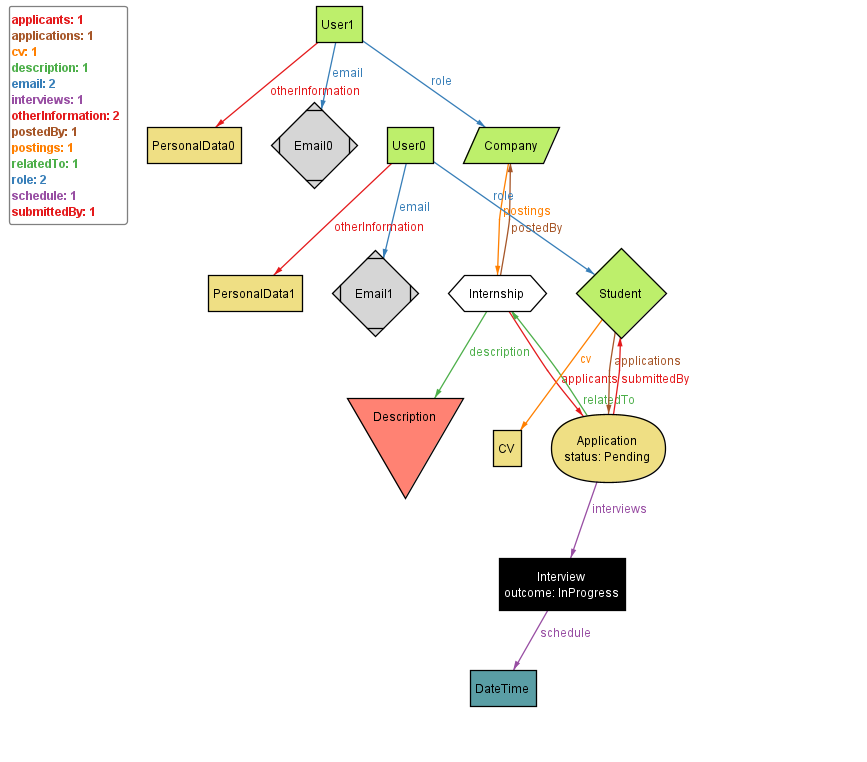
\includegraphics[width=0.75\linewidth]{RASD//Images/1st1com.png}
    \caption{1 Student, 1 Company, 1 Internship}
    \label{fig:enter-label}
\end{figure}

\textbf{[MS2]} The model shows a scenario where two students are applying for an internship at a company with pending status and an in-progress interview.
\begin{lstlisting}
//two students and one company
pred twoStudentOneCompanyOneInternship {
    #Student = 2
    #Company = 1
    #Internship = 1
}
run twoStudentOneCompanyOneInternship for 3
\end{lstlisting}
\textit{ \#7:Instance found twoStudentOneCompanyOneInternship is consistent.}
\begin{figure}[H]
    \centering
    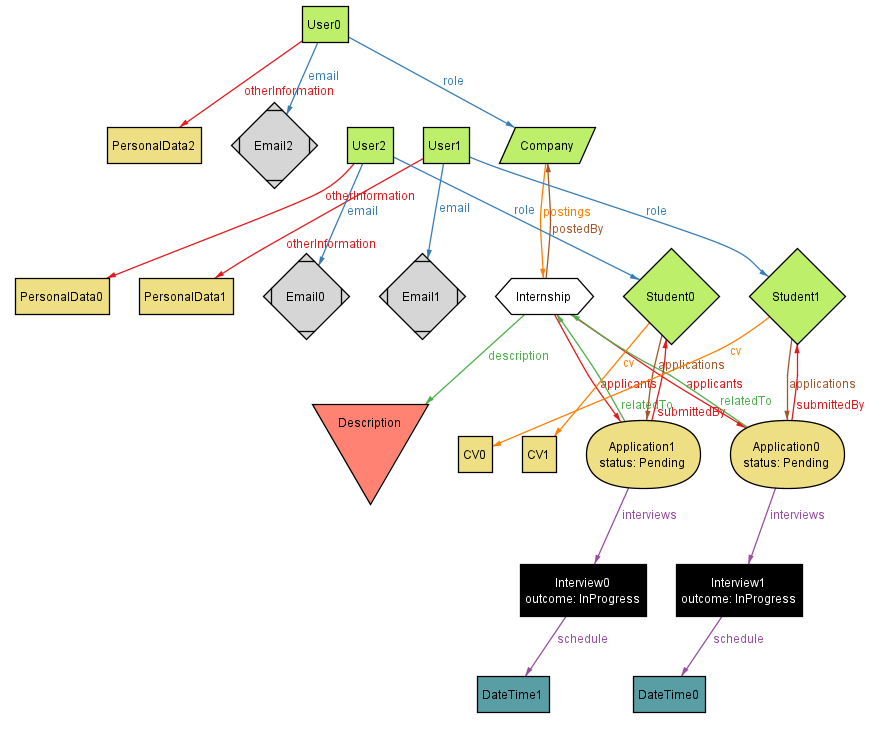
\includegraphics[width=1\linewidth]{RASD//Images/2st1com.png}
    \caption{2 Student, 1 Company, 1 Internship}
    \label{fig:enter-label}
\end{figure}

\textbf{[MS3]} The model shows a scenario where one student is applying for three internships 2 at company A and one at company B with pending status and an in-progress interview.
\begin{lstlisting}
//one student and one two companies
pred oneStudentTwoCompanyThreeInternship {
    #Student = 1
    #Company = 2
    #Internship = 3
}
run oneStudentTwoCompanyThreeInternship for 3 
\end{lstlisting}
{ \#8:Instance found oneStudentTwoCompanyThreeInternship is consistent.}
\begin{figure}[H]
    \centering
    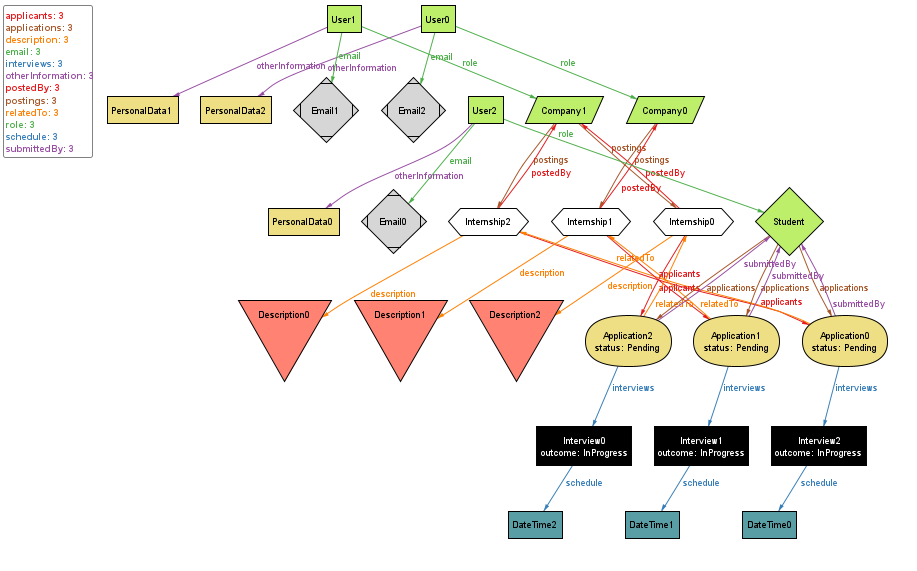
\includegraphics[width=1\linewidth]{RASD//Images/1st2com.png}
    \caption{1 Student, 1 Company, 3 Application}
    \label{fig:enter-label}
\end{figure}
\begin{figure}[H]
    \centering
    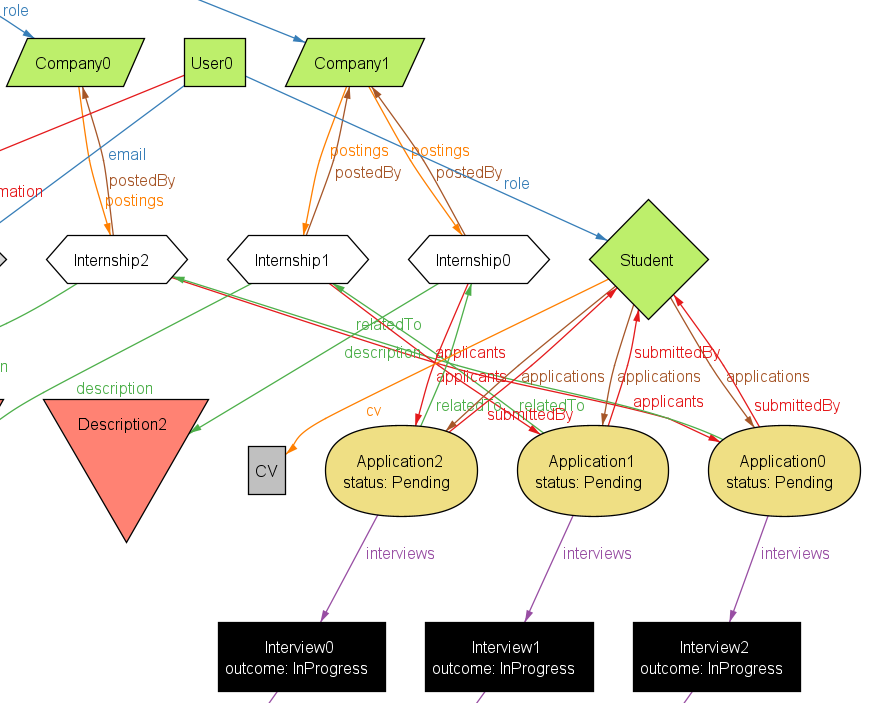
\includegraphics[width=0.75\linewidth]{RASD//Images/1st2comzoom.png}
    \caption{1 Student, 1 Company, 3 Application - zoom on the relations}
    \label{fig:enter-label}
\end{figure}

\subsection{Dynamic Analysis}
\textbf{[MD1]}The model shows the basic scenario where one student applies for an internship
at a company. The dynamic analysis shows how the positive interview status influences the application outcome.

If InProgress $=>$ Passed then Pending $=>$ Accepted
\begin{lstlisting}
//passed interview
pred interviewPassed[ap:Application, s:Student, c:Company]{
	ap.interviews.outcome = InProgress ; 
	ap.interviews.outcome = Passed
	#Student = 1
    	#Company = 1
    	#Internship = 1
}
run interviewPassed for 2  
\end{lstlisting}
{ \#9:Instance found interviewPassed is consistent.}
\begin{figure}[H]
    \centering
    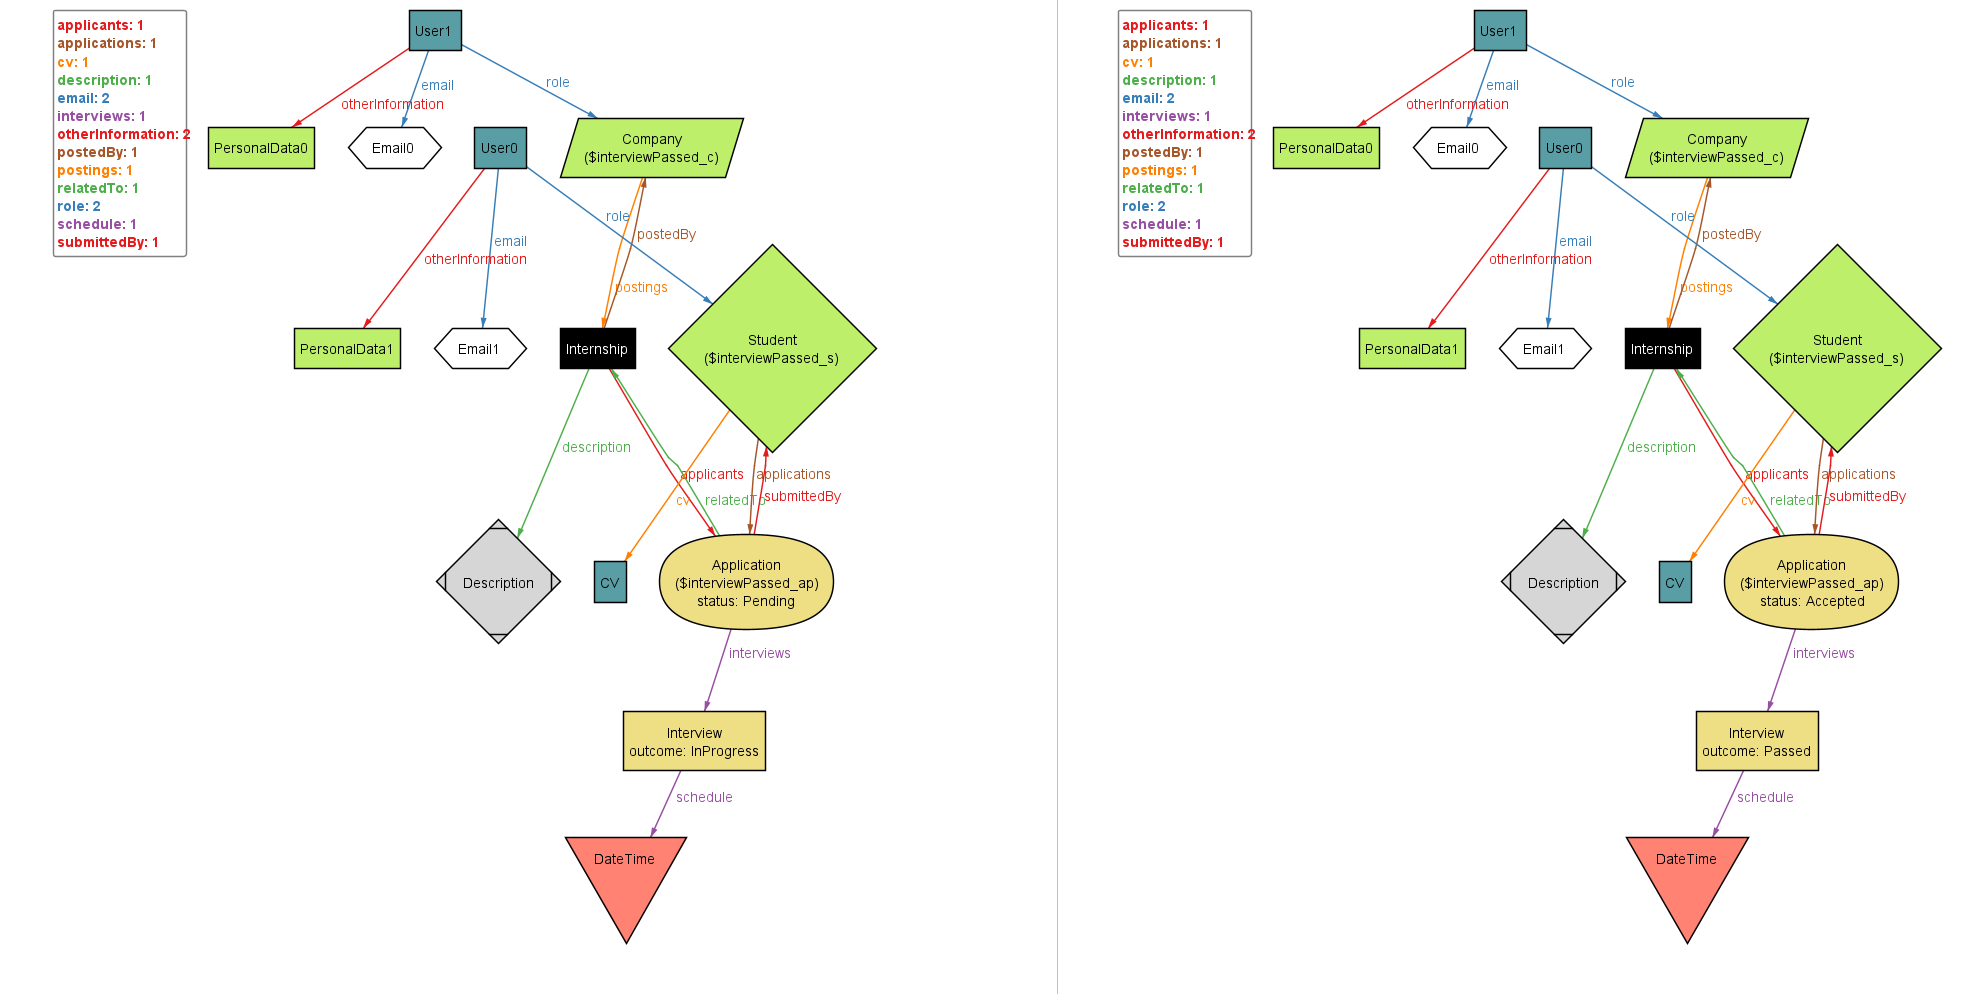
\includegraphics[width=1\linewidth]{RASD//Images/passed.png}
    \caption{Passed inteview}
    \label{fig:enter-label}
\end{figure}

\textbf{[MD2]}The model shows the basic scenario where one student applies for an internship
at a company. The dynamic analysis shows how the negative interview status influences the application outcome.

If InProgress $=>$ Failed then Pending $=>$ Rejected
\begin{lstlisting}

//failed interview
pred interviewRejected[ar:Application, s:Student, c:Company]{
	ar.interviews.outcome = InProgress ; 
	ar.interviews.outcome = Failed
	#Student = 1
    	#Company = 1
    	#Internship = 1
}
run interviewRejected for 2 
\end{lstlisting}
{ \#10:Instance found interviewRejected is consistent.}
\begin{figure}[H]
    \centering
    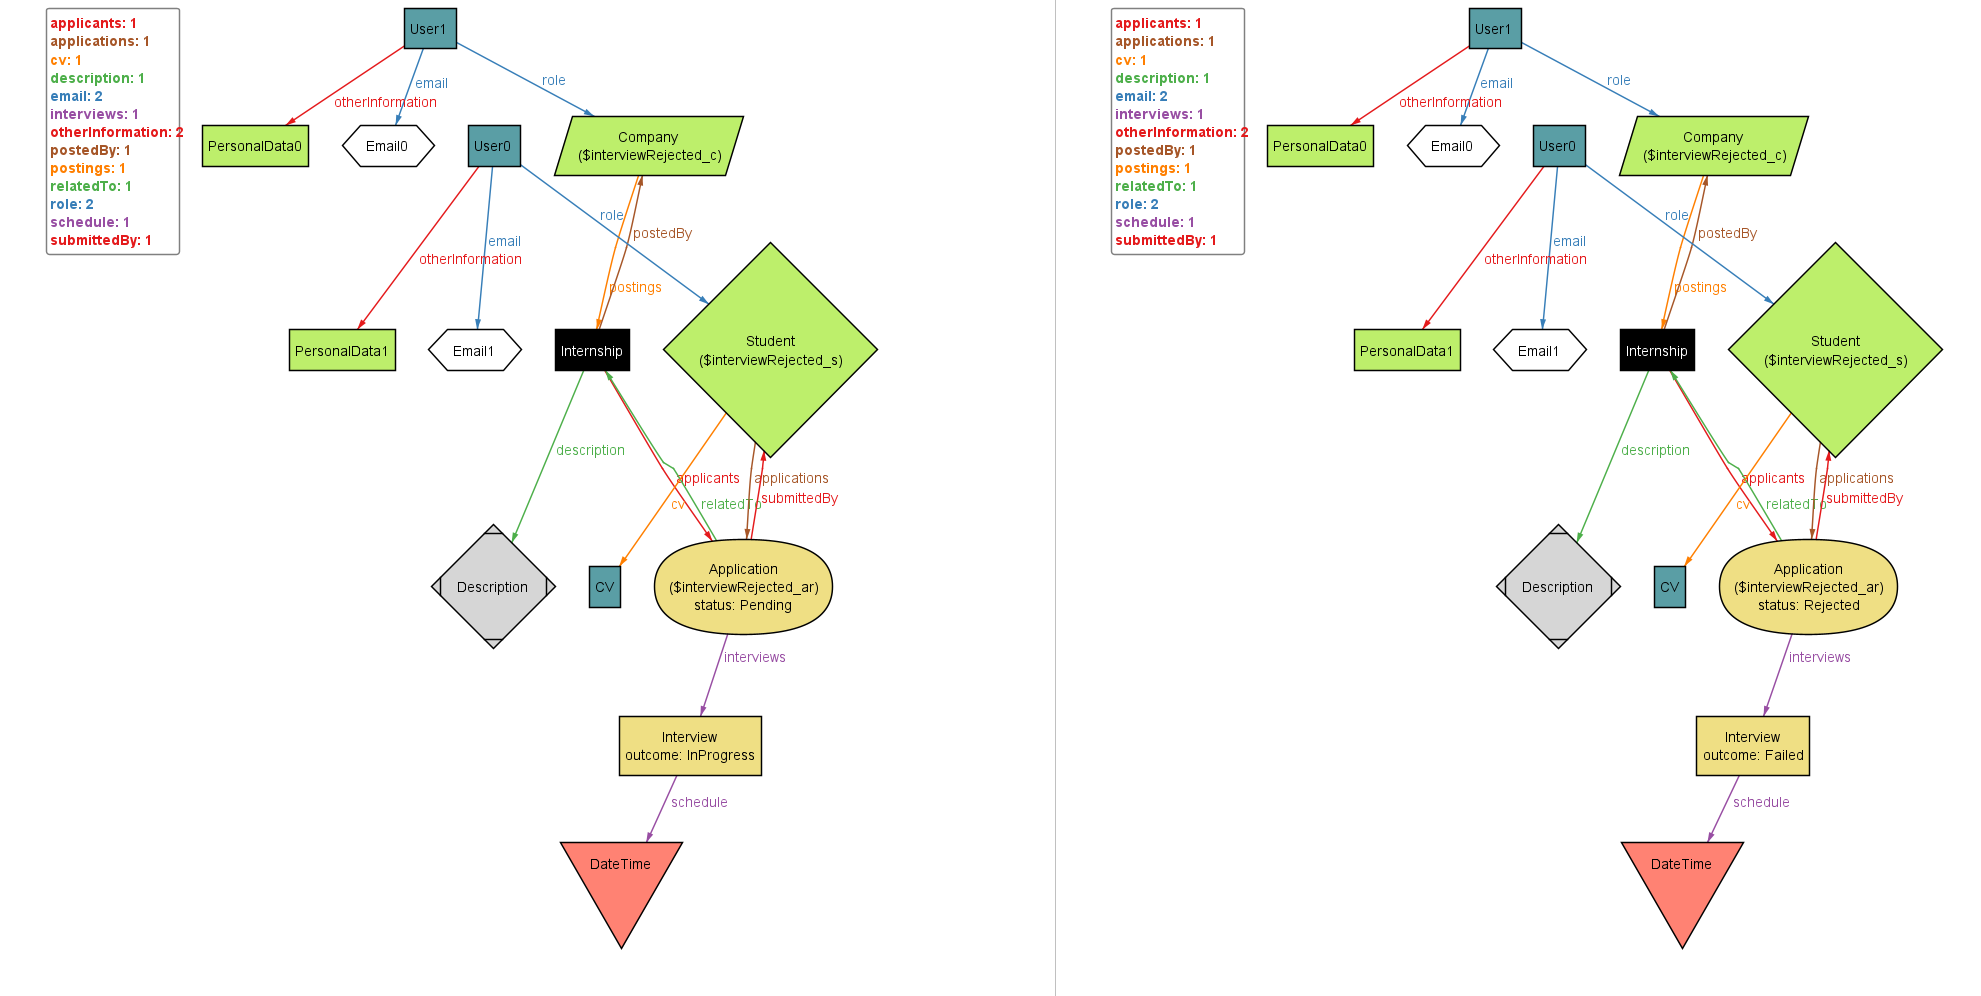
\includegraphics[width=1\linewidth]{RASD//Images/failed.png}
    \caption{Failed interview}
    \label{fig:enter-label}
\end{figure}

\section{ Assertions}
\textbf{[A1]} Assertion to verify the correctness of the user structure as:
\begin{itemize}
    \item No Users will have the same email or the Personal info
    \item Each role can only be associated with one User
\end{itemize}
\begin{lstlisting}
// Assertion to verify the correctness of the user structure as:
assert VerifyUserStructure{
	//mail and personal info
    	all u1, u2: User | u1 != u2 implies 
    		u1.email != u2.email and  
		u1.otherInformation != u2.otherInformation
	//role
    	all s: Student | one u: User | u.role = s
    	all c: Company | one u: User | u.role = c
}
check VerifyUserStructure
\end{lstlisting}
\textit{\#1: VerifyUserStructure may be valid.}


\textbf{[A2]} Assertion to verify DoubleArrowConstraint:
\begin{itemize}
    \item An application can only be associated with a student
    \item An application can only be associated with a Intenship
    \item An internship can only be associated with a Company
\end{itemize}
\begin{lstlisting}
//Assertion to verify DoubleArrowConstraint
assert VerifyDoubleAssociation {
	//An application can only be associated with a student
    	all a: Application | one s: Student | 
    	s in a.submittedBy and a in s.applications and
    	s.applications.submittedBy=s
    	//An application can only be associated with a Intenship
    	all a: Application | one i: Internship | 
    	a in i.applicants and  i in a.relatedTo and
    	i.applicants.relatedTo = i
    	//An internship can only be associated with a Company
    	all  i:Internship | one c: Company | 
    	c in i.postedBy and i in c.postings and 
    	c.postings.postedBy = c  
}
check VerifyDoubleAssociation
\end{lstlisting}
\textit{\#2: VerifyDoubleAssociation may be valid.}


\textbf{[A3]} Assertion to verify all Internship application structure
\begin{itemize}
    \item Unique Description, CV, and Interview 
    \item Unique Application
    \item A student can make only an application for one internship
\end{itemize}
\begin{lstlisting}
// Assertion to verify all Internship application structure
assert VerifyInternshipStructures {
	//Unique Description, CV, and Interview 
    	all i1, i2: Internship | i1 != i2 implies 
		i1.description != i2.description
    	all dd: Description | one ii:Internship | 
		dd in ii.description
    	all s1,s2: Student| s1 != s2 implies s1.cv != s2.cv
    	all ccvv:CV | one ss: Student |  ccvv in ss.cv
    	all a1,a2: Application | a1!=a2 implies 
		a1.interviews != a2.interviews
    	all i: Interview | one a: Application |
		i in a.interviews
    	//Unique Application
   	 all i1, i2: Internship | i1 != i2 implies 
   	#(i1.applicants & i2.applicants) <= 0
   	all c1, c2: Company | c1 != c2 implies 
   	#(c1.postings & c2.postings) <= 0
   	all s1,s2: Student | s1 !=s2 implies 
    	#(s1.applications & s2.applications) <=0
   	////Student can make only 1 application for 1 internship
    	all s: Student | all i: Internship | 
    	#(s.applications & i.applicants) <= 1
}
check VerifyInternshipStructures
\end{lstlisting}
\textit{\#3: VerifyInternshipStructures may be valid}


\textbf{[A4]} Assertion to verify all Internship meeting schedules. Two meetings cannot be on the same day if:
\begin{itemize}
    \item are carried by the same company
    \item are carried by the same student
\end{itemize}
Therefore meetings have a schedule if they are submitted by a student
\begin{lstlisting}
//Two meetings cannot be in the same day if:
assert VerifyInterviewStructures {
	all ss1,ss2: Student | all cc1,cc2: Company |
   	all a1,a2: Application | a1!=a2 and
		//are carried by the same company
   		((ss1 in a1.submittedBy and 
		   ss2 in a2.submittedBy and
   		   cc1 in a1.relatedTo.postedBy and
		   cc1 in a1.relatedTo.postedBy)
   	or
		//are carried by the same student
   		 (ss1 in a1.submittedBy and 
		  ss1 in a2.submittedBy and
   		  cc1 in a1.relatedTo.postedBy and 
		  cc2 in a1.relatedTo.postedBy))
   	implies a1.interviews.schedule != a2.interviews.schedule
  	//meetings have a schedule if a student submits them
   	all a: Application | a.interviews.schedule != none 
   		 implies a.submittedBy in Student
}
check VerifyInternshipStructures
\end{lstlisting}
\textit{\#4: VerifyInterviewStructures may be valid}

\textbf{[A5]} Assertion to verify if the interview process is correctly related to the application process. Three cases are considered:
\begin{itemize}
    \item Failed $=>$ Rejected
    \item Passed $=>$ Accepted
    \item InProgress $=>$ Pending
\end{itemize}
\begin{lstlisting}
//Check interview process
assert InterviewProcess{
    all a: Application | 
	//Failed => Rejected
        some i: a.interviews | i.outcome = Failed 
		implies a.status = Rejected
	and 
	//Passed => Accepted
        some i: a.interviews | i.outcome = Passed 
		implies a.status = Accepted
	and
	//InProgress => Pending
        some i: a.interviews | i.outcome = InProgress 
		implies a.status = Pending
}
check InterviewProcess
\end{lstlisting}
\textit{\#5: InterviewProcess may be valid}

\chapter{Effort Spent}

\begin{table}[H]
    \begin{center}
        \begin{tabular}{c|c}
            \hline
            Member of group & Effort spent \\
            \hline
            Arianna Paone & \begin{tabular}{p{0.25\linewidth}|c}
                             Introduction          & $6h$  \\
                             Overall description   & $9h$ \\
                             Specific requirements & $15h$ \\
                             Formal analysis       & $2h$ \\
                             Homework              & $3h$ \\
            \end{tabular} \\
            \hline
            Matteo Pasqual & \begin{tabular}{p{0.25\linewidth}|c}
                             Introduction          & $6h$  \\
                             Overall description   & $4h$ \\
                             Specific requirements & $7h$ \\
                             Formal analysis       & $10h$  \\
                             Homework              & $3h$ \\
            \end{tabular} \\
            \hline
            Matilde Restelli & \begin{tabular}{p{0.25\linewidth}|c}
                            Introduction          & $7h$ \\
                            Overall description   & $5h$ \\
                            Specific requirements & $7h$ \\
                            Formal analysis       & $2h$ \\
                            Homework              & $3h$ \\
            \end{tabular} \\
            \hline
        \end{tabular}
        \caption{Effort spent by each member of the group.}
        \label{tab:effor_spent}
    \end{center}
\end{table}


\cleardoublepage
\end{document}